\subsection{Design}
This section describes the main aspects of the VFS core library. It shows the
implementation of the core interfaces and classes, explains the mock classes and
tests and eventually describes the file format and its management classes.

\subsubsection{Core Classes}\label{sec:coreClasses}
Figure \ref{fig:core_classes} gives an overview of the main interfaces and
classes that were implemented. The interfaces \textit{VFSDiskManager},
\textit{VFSEntry} and \textit{VFSPath} can be used by clients using the library
implemented here.
\begin{itemize}
\item{\textit{VFSDiskManager}} The implementations of this interface provide
mainly a way to open, create and dispose new virtual disks. Additionally one can
get the root entry of the file system and get additional information about an
opened disk.
\item{\textit{VFSEntry}} Represents a directory or file on the file system. A
\textit{VFSEntry} provides all the required methods to manipulate files and
directories and importing/exporting files into the virtual file system. The
general meaning of \textit{VFSEntry} is, that such objects usually exist on the
filesystem.
\item {\textit{VFSPath}} Represents a path on the file system to a given
\textit{VFSEntry}. It has a slightly looser coupling to the file system as a
path does not imperatively need to exist.
\end{itemize}

The intention of those interfaces is to hide the real implementation of the
virtual file system from a client. With that in mind it should be simple to add
a network layer upon the real implementation without changing client code. The
classes \textit{VFSDiskManagerImpl, VFSEntryImpl (and its descendants) and
VFSPathImpl} implement all the management for actually using the VFS on a virtual disk.

\begin{figure}[h!]
\centering
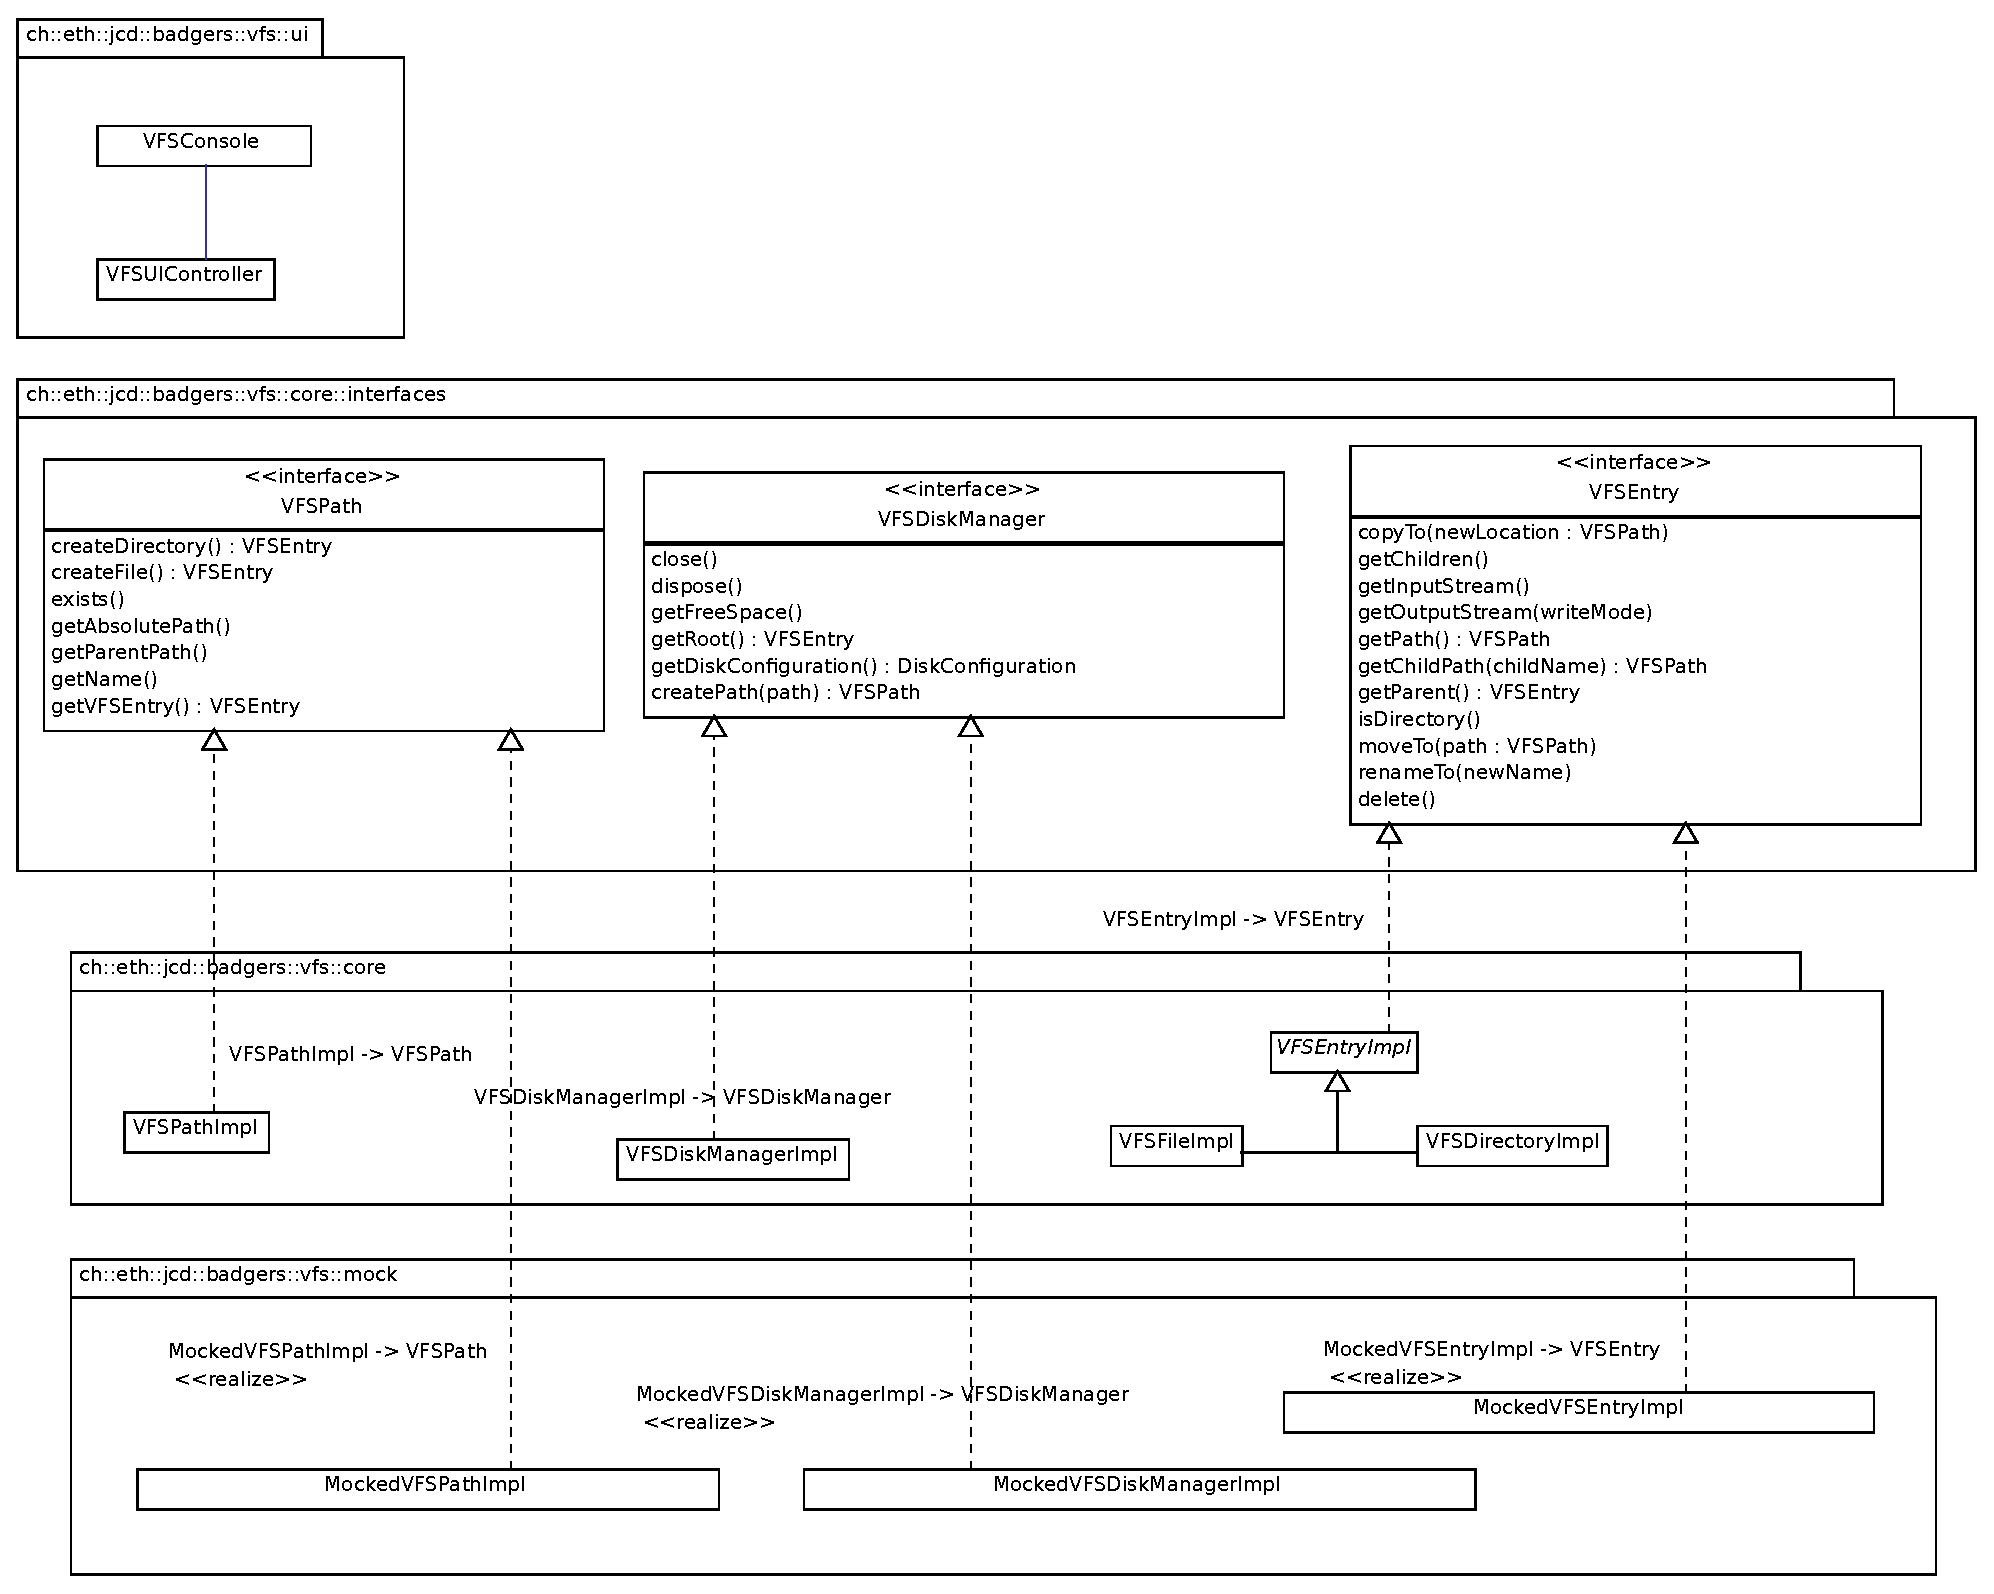
\includegraphics[width=1\textwidth]{figures/core_classes.eps}
\caption{core classes}
\label{fig:core_classes}
\end{figure}

\subsubsection{Mocking}
For discussing the semantics of the virtual file system and the development of 
the interfaces explained in \ref{sec:coreClasses} it was decided to implement a mock
that works against the host file system. The mock classes implement all
the interfaces and were very helpful for acquiring a common understanding of how
the interface shall be used by clients. In a further step it was very useful to have
the mock classes while developing the console application which could be
developed independently from the real implementation.
\subsubsection{Test}
During the development a bunch of test cases came to life. The tests solely
depend on the interfaces and thus they can run against the mock classes and the
real implementation. This was a huge help in finding bugs in the slightly more
complicated real implementation.